The \textit{Repository Management} module is responsible for management and cataloging of
algorithms and test data to be used in the benchmarking tests.

\subsection{Domain Model}
The domain model for the Repository Management module is shown in Figure \ref{fig:repoManDomain}
\begin{figure}[H]
  \begin{center}
  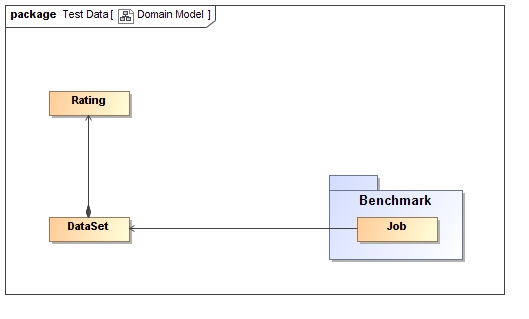
\includegraphics[scale=0.5]{../Diagrams and Charts/Test Data/Domain Model.jpg}  
  \caption{Repository Management Domain Model}
  \label{fig:repoManDomain}
  \end{center}  
\end{figure}
\clearpage
\subsection{Scope}
The scope for the Repository Management module is shown in Figure \ref{fig:repoManScope}
\begin{figure}[H]
  \begin{center}
  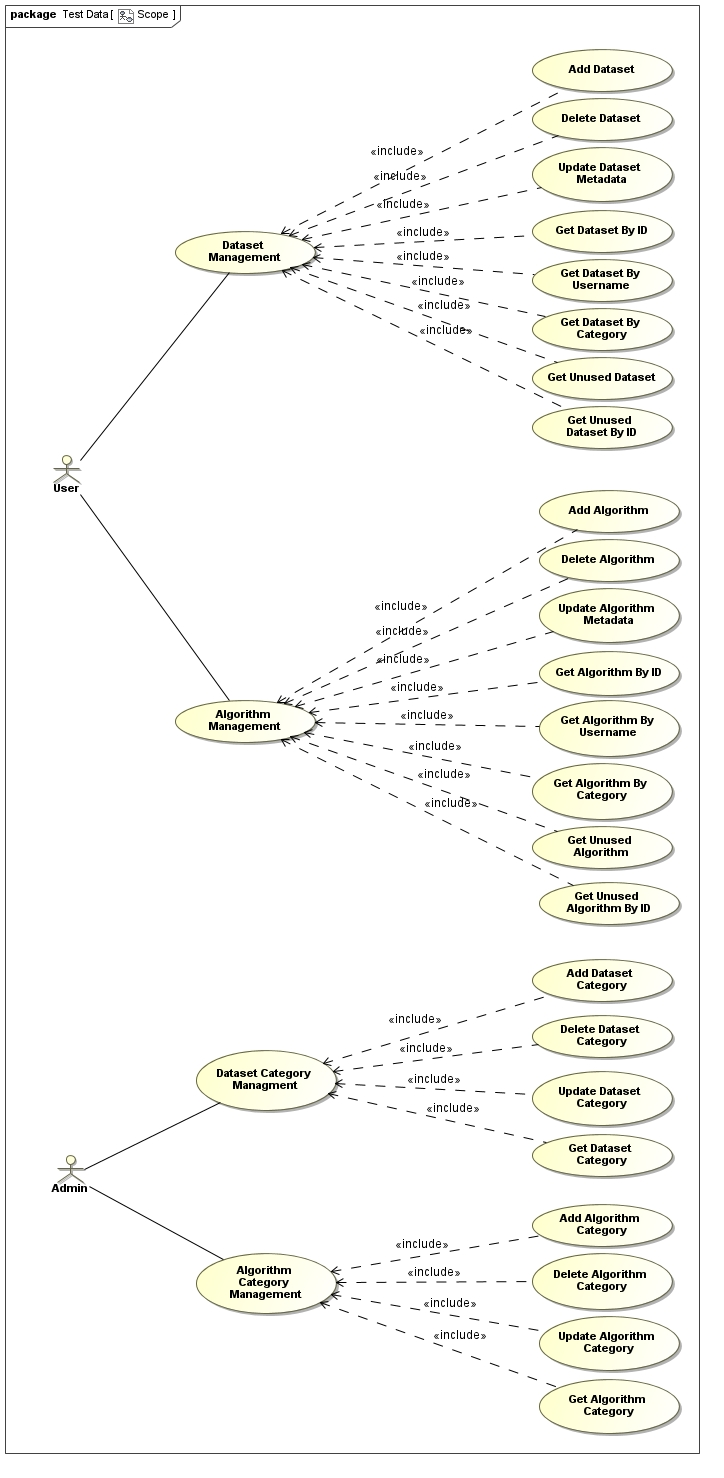
\includegraphics[scale=0.3]{../Diagrams and Charts/Test Data/Scope.jpg}
  \caption{Scope of Categories}
  \label{fig:repoManScope}
  \end{center}  
\end{figure}

\subsection{Dataset Management}

\subsubsection {Add dataset}
The service contract for adding a dataset is shown in Figure \ref{fig:addDatasetService}
\begin{figure}[H]
  \begin{center}
  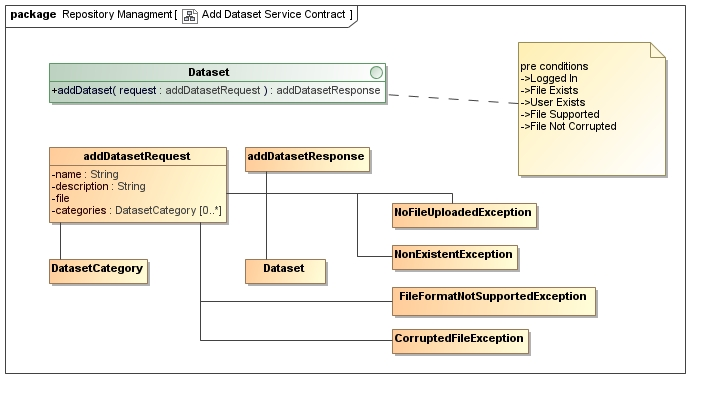
\includegraphics[scale=0.6]{../Diagrams and Charts/Test Data/Add Dataset Service Contract.jpg}
  \caption{Add Dataset Service Contract}
  \label{fig:addDatasetService}
  \end{center}  
\end{figure}

\subsubsection {Delete dataset}
\subsubsection {Update dataset}
\subsubsection {Get dataset by ID}
\subsubsection {Get dataset by name}
\subsubsection {Get dataset by category}
\subsubsection {Get unused datasets}
\subsubsection {Get unused dataset by ID}

\subsection{Algorithm Management}
\subsubsection {Users will be able to add an algorithm}
\paragraph{Service Contract}
The service contract for adding an algorithm is shown in Figure \ref{fig:addAlgorithmService}

\begin{figure}[H]
  \begin{center}
  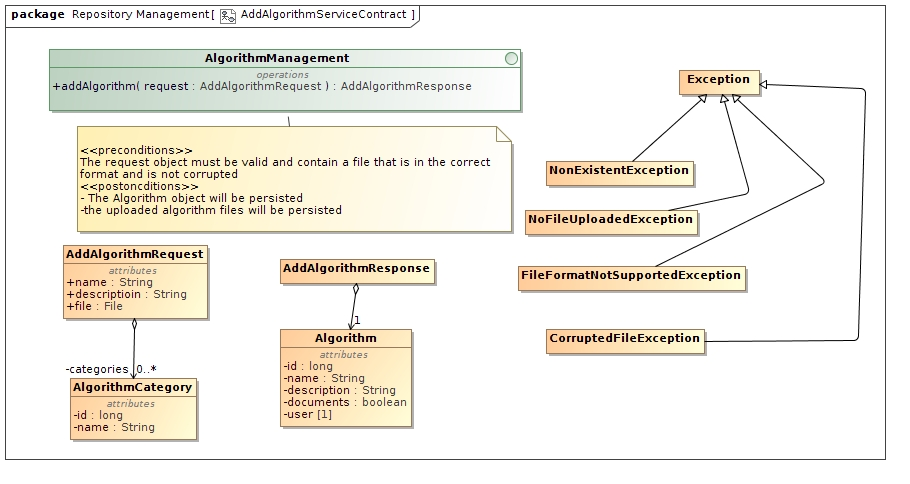
\includegraphics[scale=0.5]{../Diagrams and Charts/Test Data/AddAlgorithmServiceContract.jpg}
  \caption{Add Algorithm Service Contract}
  \label{fig:addAlgorithmService}
  \end{center}  
 \end{figure}

 The service will add the Algorithm meta data as well as the store the
 actual Algorithm files to a database.\\\\
 The service will be refused if:\\
	 \begin{itemize}
	 	\item The request object does not have a valid structure.	 	
	 	\item The request object does not contain a file.
	 	\item The file is not in an acceptable format
	 	\item The file is corrupted
	 \end{itemize}
In each case the appropriate exception will be thrown.

\subsubsection {Users will be able to delete an algorithm}
\paragraph{Service Contract}
The service contract for deleting an algorithm is shown in Figure \ref{fig:deleteAlgorithmService}

\begin{figure}[H]
  \begin{center}
  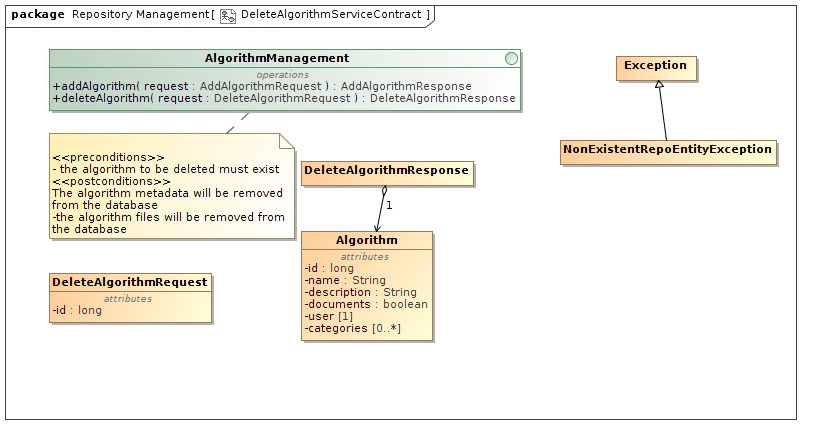
\includegraphics[scale=0.5]{../Diagrams and Charts/Test Data/DeleteAlgorithmServiceContract.jpg}
  \caption{Delete Algorithm Service Contract}
  \label{fig:deleteAlgorithmService}
  \end{center}  
 \end{figure}

 The service will delete the Algorithm meta data as well as the stored files
 of the actual Algorithm.\\\\
 The service will be refused if:\\
	 \begin{itemize}
	 	\item The Algorithm to be deleted does not exist.
	 \end{itemize}
In this case a NonExistentRepoEntityException will be thrown.

\paragraph{Functional Requirements}
Figure \ref{fig:deleteAlgorithmFuncReq} shows the lower level services required
by the deleteAlgorithm service to either check the pre-conditions or address the
post-conditions.

\begin{figure}[H]
  \begin{center}
  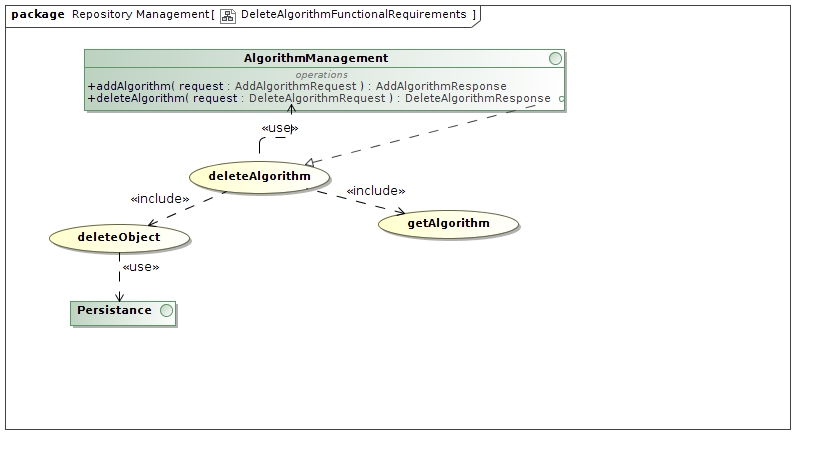
\includegraphics[scale=0.5]{../Diagrams and Charts/Test Data/DeleteAlgorithmFunctionalRequirements.jpg}
  \caption{Delete Algorithm Functional Requirements}
  \label{fig:deleteAlgorithmFuncReq}
  \end{center}  
 \end{figure}

 The service will first try to get the Algorithm to be deleted to see if it
 exists. If it does it will use a persistance interface to delete the object
 from the repository.

\subsubsection {Users will be able to update an algorithm}
\subsubsection {Users will be able to get an algorithm by ID}
\subsubsection {Users will be able to get an algorithm by name}
\subsubsection {Users will be able to get an algorithm by category}
\subsubsection {Users will be able to get all unused algorithms}
\subsubsection {Users will be able to get an unused algorithm by ID}

\subsection{Dataset Category Management}

\subsubsection {Add dataset category}
The service contract for adding a dataset category is shown in Figure \ref{fig:addDatasetCatService}
\begin{figure}[H]
  \begin{center}
  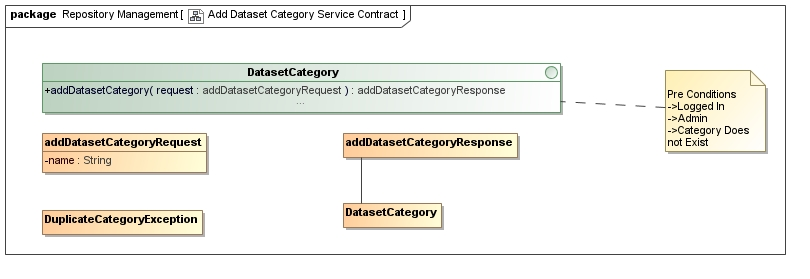
\includegraphics[scale=0.6]{../Diagrams and Charts/Test Data/Add Dataset Category Service Contract.jpg}
  \caption{Add Dataset Category Service Contract}
  \label{fig:addDatasetCatService}
  \end{center}
  
\end{figure}

The pre-conditions
\begin{itemize}
  \item User needs to be an admin
  \item All details of the new dataset category need to be valid
  \item Category must not exist
\end{itemize}

The post-conditions
\begin{itemize}
  \item Category is created succesfully
\end{itemize}

\subsubsection {Delete dataset category}

The service contract for deleting a dataset category is shown in Figure \ref{fig:deleteDatasetCatService}
\begin{figure}[H]
  \begin{center}
  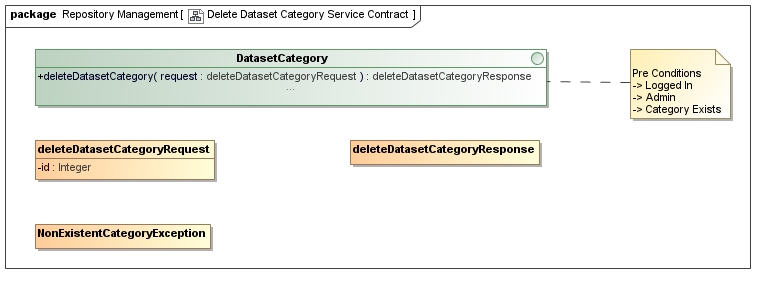
\includegraphics[scale=0.6]{../Diagrams and Charts/Test Data/Delete Dataset Category Service Contract.jpg}
  \caption{Delete Dataset Category Service Contract}
  \label{fig:deleteDatasetCatService}
  \end{center}
  
\end{figure}

The pre-conditions
\begin{itemize}
  \item User needs to be an admin
  \item Category must exist
  \item No dataset must be assigned to this category
\end{itemize}

The post-conditions
\begin{itemize}
  \item Category is deleted succesfully
\end{itemize}

\subsubsection {Update dataset category}

The service contract for updating a dataset category is shown in Figure \ref{fig:updateDatasetCatService}
\begin{figure}[H]
  \begin{center}
  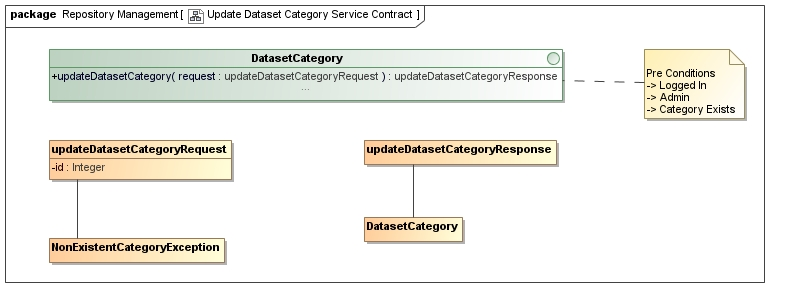
\includegraphics[scale=0.6]{../Diagrams and Charts/Test Data/Update Dataset Category Service Contract.jpg}
  \caption{Update Dataset Category Service Contract}
  \label{fig:updateDatasetCatService}
  \end{center}
  
\end{figure}


The pre-conditions
\begin{itemize}
  \item User needs to be an admin
  \item Category must exist
  \item New details must be valid
\end{itemize}

The post-conditions
\begin{itemize}
  \item Category is updated succesfully
\end{itemize}
\subsubsection {Get dataset category}

The service contract for getting a dataset category is shown in Figure \ref{fig:getDatasetCatService}
\begin{figure}[H]
  \begin{center}
  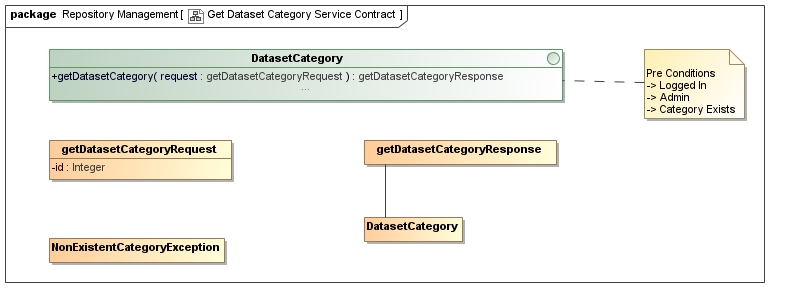
\includegraphics[scale=0.6]{../Diagrams and Charts/Test Data/Get Dataset Category Service Contract.jpg}
  \caption{Get Dataset Category Service Contract}
  \label{fig:getDatasetCatService}
  \end{center}
  
\end{figure}

The pre-conditions
\begin{itemize}
  \item Category must exist
\end{itemize}

The post-conditions
\begin{itemize}
  \item Category is gotten succesfully
\end{itemize}

\subsubsection{Get Dataset By Username}
The service contract for getting a dataset by username is shown in Figure \ref{fig:getDatasetByUsername}
\begin{figure}[H]
	\begin{center}
		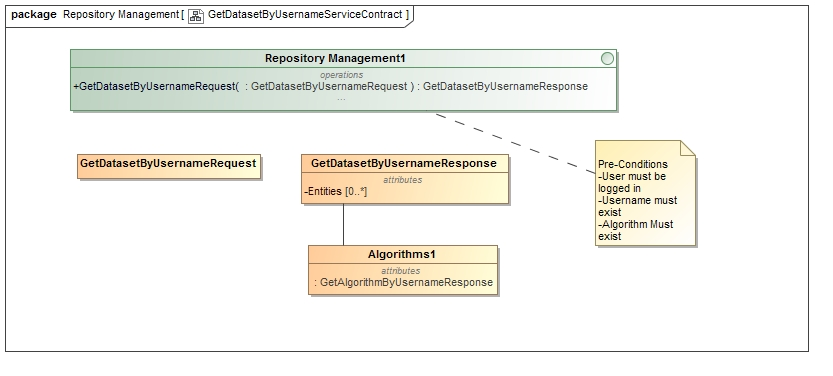
\includegraphics[scale=0.6]{../Diagrams and Charts/Test Data/GetDatasetByUsernameServiceContract.jpg}
		\caption{Get Dataset By Username Service Contract}
		\label{fig:getDatasetByUsername}
	\end{center}
	
\end{figure}	

The pre-conditions
\begin{itemize}
	\item User must be logged in.
	\item Username must exist.
	\item Dataset must exist.
\end{itemize}

The post-conditions
\begin{itemize}
	\item Dataset is successfully retrieved.
\end{itemize}

\subsubsection{Get Unused Dataset By Username}
The service contract for getting an unused dataset by username is shown in Figure \ref{fig:getUnusedDatasetByUsername}
\begin{figure}[H]
	\begin{center}
		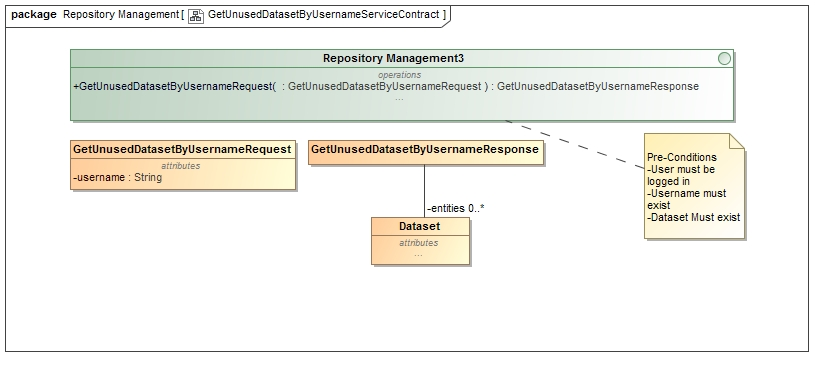
\includegraphics[scale=0.6]{../Diagrams and Charts/Test Data/GetUnusedDatasetByUsernameServiceContract.jpg}
		\caption{Get an Unused Dataset By Username Service Contract}
		\label{fig:getUnusedDatasetByUsername}
	\end{center}
	
\end{figure}	

The pre-conditions
\begin{itemize}
	\item User must be logged in.
	\item Username must exist.
	\item Dataset must exist.
\end{itemize}

The post-conditions
\begin{itemize}
	\item Dataset is successfully retrieved.
\end{itemize}

\subsection{Algorithm Category Management}

\subsubsection {Add algorithm category}
The service contract for adding a algorithm category is shown in Figure \ref{fig:addAlgorithmCatService}
\begin{figure}[H]
  \begin{center}
  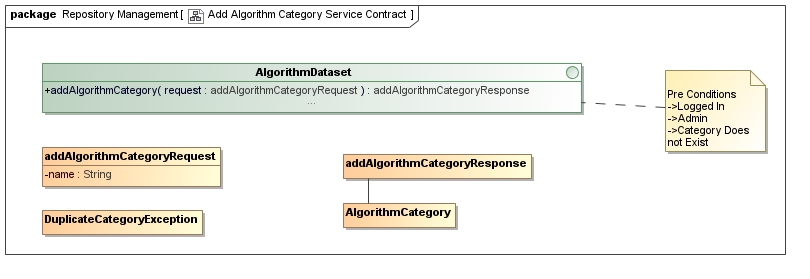
\includegraphics[scale=0.6]{../Diagrams and Charts/Test Data/Add Algorithm Category Service Contract.jpg}
  \caption{Add Algorithm Category Service Contract}
  \label{fig:addAlgorithmCatService}
  \end{center}
  
\end{figure}

The pre-conditions
\begin{itemize}
  \item User needs to be an admin
  \item All details of the new algorithm category need to be valid
  \item Category must not exist
\end{itemize}

The post-conditions
\begin{itemize}
  \item Category is created succesfully
\end{itemize}

\subsubsection {Delete algorithm category}

The service contract for deleting a algorithm category is shown in Figure \ref{fig:deleteAlgorithmCatService}
\begin{figure}[H]
  \begin{center}
  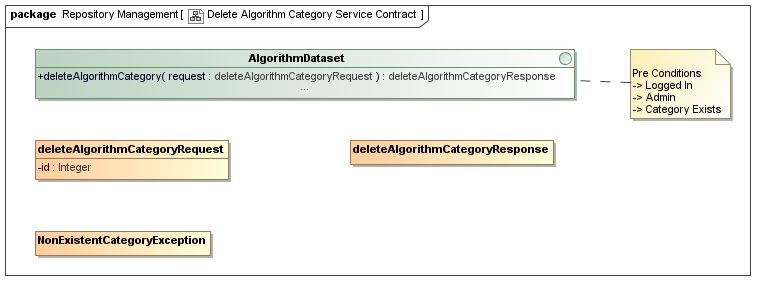
\includegraphics[scale=0.6]{../Diagrams and Charts/Test Data/Delete Algorithm Category Service Contract.jpg}
  \caption{Delete Algorithm Category Service Contract}
  \label{fig:deleteAlgorithmCatService}
  \end{center}
  
\end{figure}

The pre-conditions
\begin{itemize}
  \item User needs to be an admin
  \item Category must exist
  \item No algorithm must be assigned to this category
\end{itemize}

The post-conditions
\begin{itemize}
  \item Category is deleted succesfully
\end{itemize}

\subsubsection {Update algorithm category}

The service contract for updating a algorithm category is shown in Figure \ref{fig:updateAlgorithmCatService}
\begin{figure}[H]
  \begin{center}
  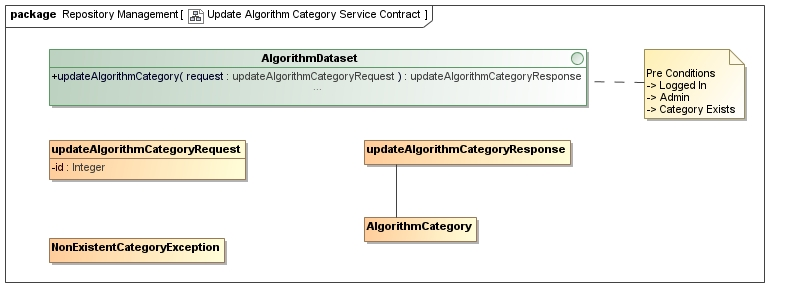
\includegraphics[scale=0.6]{../Diagrams and Charts/Test Data/Update Algorithm Category Service Contract.jpg}
  \caption{Update Algorithm Category Service Contract}
  \label{fig:updateAlgorithmCatService}
  \end{center}
  
\end{figure}


The pre-conditions
\begin{itemize}
  \item User needs to be an admin
  \item Category must exist
  \item New details must be valid
\end{itemize}

The post-conditions
\begin{itemize}
  \item Category is updated succesfully
\end{itemize}
\subsubsection {Get algorithm category}

The service contract for getting a algorithm category is shown in Figure \ref{fig:getAlgorithmCatService}
\begin{figure}[H]
  \begin{center}
  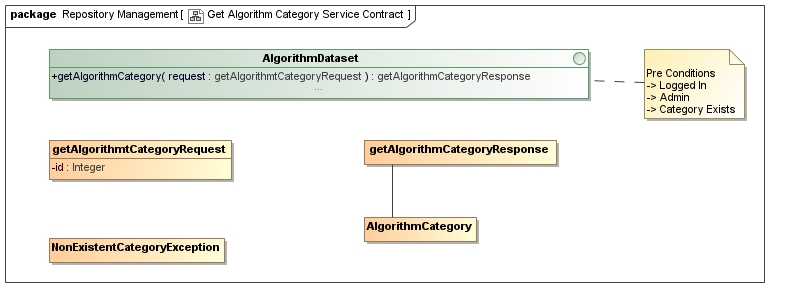
\includegraphics[scale=0.6]{../Diagrams and Charts/Test Data/Get Algorithm Category Service Contract.jpg}
  \caption{Get Algorithm Category Service Contract}
  \label{fig:getAlgorithmCatService}
  \end{center}
  
\end{figure}

The pre-conditions
\begin{itemize}
  \item Category must exist
\end{itemize}

The post-conditions
\begin{itemize}
  \item Category is gotten succesfully
\end{itemize}

\subsubsection{Get Algorithm By Username}
The service contract for getting an algorithm by username is shown in Figure \ref{fig:getAlgorithmByUsername}
\begin{figure}[H]
	\begin{center}
		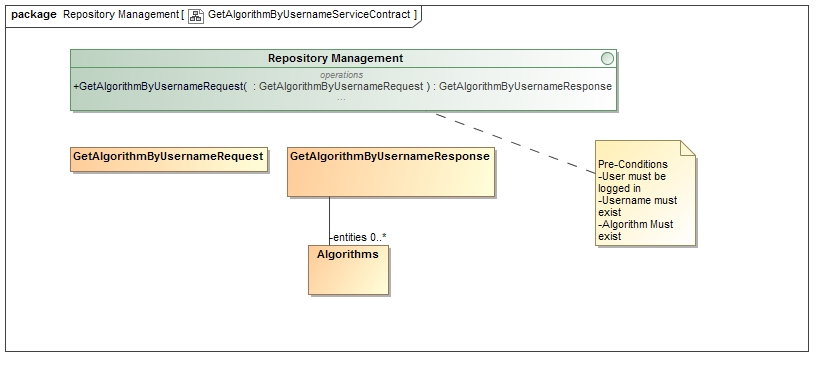
\includegraphics[scale=0.6]{../Diagrams and Charts/Test Data/GetAlgorithmByUsernameServiceContract.jpg}
		\caption{Get Algorithm By Username Service Contract}
		\label{fig:getAlgorithmByUsername}
	\end{center}
	
\end{figure}	

The pre-conditions
\begin{itemize}
	\item User must be logged in.
	\item Username must exist.
	\item Algorithm must exist.
\end{itemize}

The post-conditions
\begin{itemize}
	\item Algorithm is successfully retrieved.
\end{itemize}

\subsubsection{Get Unused Algorithm By Username}
The service contract for getting an unused algorithm by username is shown in Figure \ref{fig:getUnusedAlgorithmByUsername}
\begin{figure}[H]
	\begin{center}
		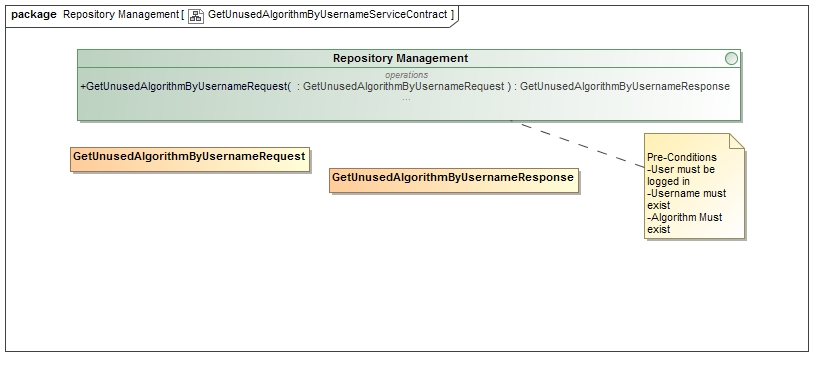
\includegraphics[scale=0.6]{../Diagrams and Charts/Test Data/GetUnusedAlgorithmByUsernameServiceContract.jpg}
		\caption{Get an Unused Algorithm By Username Service Contract}
		\label{fig:getUnusedAlgorithmByUsername}
	\end{center}
	
\end{figure}	

The pre-conditions
\begin{itemize}
	\item User must be logged in.
	\item Username must exist.
	\item Algorithm must exist.
\end{itemize}

The post-conditions
\begin{itemize}
	\item Algorithm is successfully retrieved.
\end{itemize}





